\section{The Plasticine Architecture and its Programming Interface}

\begin{figure*}
\centering
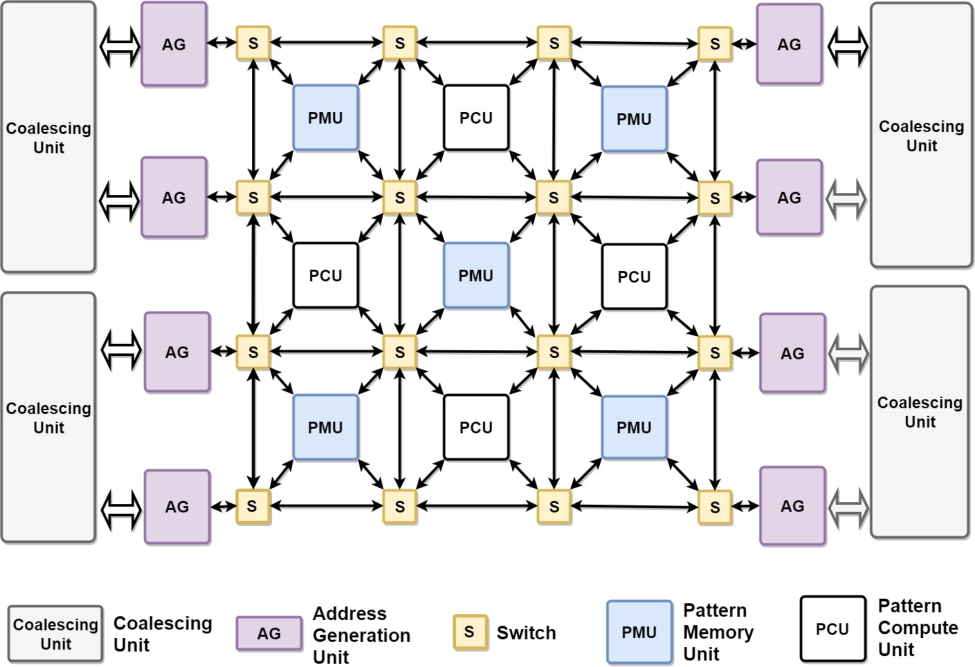
\includegraphics[width=0.7\textwidth]{figs/plasticine.pdf}
\caption[Plasticine chip-level architecture]{Plasticine chip-level architectural diagram}
\label{fig:plasticine}
\end{figure*}

%Like high-level synthesis tools for FPGAs, \name starts with a high-level imperative programming
%abstraction and synthesizes the program to execute on a reconfigurable accelerator. Targeting an \rda, however,
%is more challenging than targeting FPGAs, due to \rda's stringent mapping constraints. 
%Unlike FPGAs, \rdas cannot map arbitrary RTL functionality. 

%Taking Plasticine as an example, 
%the hardware has a collection of memory tiles (PMUs) and compute tiles (PCUs). 
Plasticine is a tile-based reconfigurable dataflow accelerator designed for a wide range of data-intensive
workloads.
With an area footprint of $113mm^2$ at 28-nm process, Plasticine packs 12.3 TFLOPS of compute
throughput and 16 MB of on-chip memory. 
Without bit-level reconfiguration overhead,
Plasticine runs a higher clock frequency than most FPGAs, running at 1GHz 
with a thermal design power at 49W. 
Previous work has shown a up to 77X performance-per-watt improvement from Plasticine over a Stratix
V FPGA~\cite{plasticine}.
\Cref{fig:plasticine} shows the chip-level design of Plasticine.

At high-level, Plasticine contains an array of resource tiles connected by a global interconnect.
The mesh network is statically configured, providing a guaranteed in-order transmission
of packet streams between any tiles.
The network comes with three granularity: a 512-bit vector data bus, a 32-bit scalar data bus, and a
single-bit control bus.
The data networks contain a single valid bit traveled along with the data;
the control network has only the valid bit without a payload, transmitting control pulses across tiles.
There are three types of configurable units: the pattern compute units (PCUs) perform the most
heavy lifting computation on Plasticine; the pattern memory units (PMUs) contain all distributed
scratchpad on-chip; and the DRAM Address Generation Unit (AG) that generates DRAM requests going to
the off-chip memory.

Like FPGAs, Plasticine can also support multiple-level of parallelization and pipelining explained
in the previous section.

For the rest of this section, we will explain the native programming interfaces of the three
configurable units.

\subsubsection{Pattern Compute Unit (PCU)}
As the major compute workhorse of the architecture, a PCU contains a 6-stage SIMD pipeline with 16 SIMD lanes. 
Unlike a processor core, the PCU can only statically configure six vector instructions throughout the
entire execution.
Additionally, the six instructions must be branch-free in order to be fully pipelined across stages.
At runtime, the SIMD pipeline executes the same set of instructions over different input data.
The software can configure the SIMD pipeline to depend on a set of input streams and
produce a set of output streams. 
There are three types of streams---single-bit control streams, 32-bit word scalar streams, and
16-word vector streams---corresponding to three types of global networks.
Execution of the PCU is triggered by the arrival of its input dependencies and back pressured by
the downstream buffers.
PCU also contains configurable counters, which can be chained to produce the values of nested
loop iterators used in the datapath. 

\begin{figure}
  \begin{subfigure}[b]{0.5\textwidth}
    \inputminted{python}{code/contextfull.py}
    \caption{Declarative configuration}
    \label{fig:contexta}
  \end{subfigure}
  \hfill
  \begin{subfigure}[b]{0.4\textwidth}
    \inputminted{python}{code/context_dec_simple.py}
    \caption{Declarative configuration with automatic register allocation}
    \label{fig:contextb}
    \inputminted{python}{code/context_imp.py}
    \caption{Equivalent imperative program}
    \label{fig:contextc}
  \end{subfigure}
  \caption[Example PCU configuration]{
    Pseudo PCU configuration.
    (a) shows the simplified declarative-style configuration for the SIMD pipeline context in a PCU.
    Each PCU context can produce a set of output streams as a function of input streams and counter
    values.
    Each stage contains multiple pipeline registers (PRs) that can propogate results across stages.
    A stage can read PRs from the previous stage and write to PRs in its current stage.
    Only the first stage can read streams and counter values and the last stage can write streams. 
    Other stages need to propogate the required values through PRs.
    (b) shows a simplified configuration where registers are implicitly allocated.
    By configuring when each stream is enqueued and dequeued using signals from the chained counters, 
    these streams are effectively read and written within different loop bodies.
    (c) shows the effective execution achieved in an imperative program.
    In (b), the \texttt{valid} signal of the inner most counter \texttt{j} is high whenever the context is
    enabled. The context is implicitly triggered whenever its input streams \texttt{streamA},
    \texttt{streamB}, and \texttt{streamC} are non-empty and output stream \texttt{outputD} is ready.
    %The declarative configuration also specifies a pipeline register (PR) to holds output of each stage
    %and explicitly forward live variables across stages. 
    %For simplicity, these details are omitted in the imperative-style on the right and
    %\Cref{sec:regalloc} gives more details on register allocation for the SIMD pipeline.
    In (b) and (c), we move the definitions of streams outside of the context, so they can be written by
    other contexts. 
    Each stream can have exactly one writer. 
    If a stream has more than one reader, effectively the
    writer broadcasts the result to both input buffers of the receiver contexts.
  }
  \label{fig:context}
\end{figure}

We refer to the program graph that can be executed by the SIMD pipeline as a \term{compute context} or
simply \term{context}. 
A context includes the branch-free instructions mapped across SIMD stages, the input and output streams, and associated counter states and control configurations.
\Cref{fig:contexta} shows an example of a simplified pseudo assembly code to program a PCU context.
The control signals of the configurable counters, such as counter saturation or \term{counter done}
signals, can be used to dequeue and enqueue the input and output streams, respectively.
The counter bounds (i.e., min, max, and stride) can also be data-dependent using values from the scalar input streams. Compared to other dataflow architectures, the dataflow engine in Plasticine is more flexible in that it allows dynamic enqueue and dequeue window for its input and output streams.
\emph{This feature enables Plasticine to support complex control hierarchy, such as non-perfectly nested loops and
branch statements, across contexts even though individual contexts can only execute instructions that are
control-free}. 

\Cref{fig:contextc} represents the effective execution achieved in an imperative-style program.
For simplicity, we will use the imperative-style configuration in the later discussion.
However, it is important to realize the instructions in the imperative-style configurations are not
executed in time, but rather in space.
There is a one-to-one translation from the declarative-style configuration to the imperative-style, but not in a reverse way.
%There are many restrictions on the structure of the program in the imperative-style. 
Instructions in the contexts must belongs to a single basic block, and the loops need to be
perfectly nested (only accesses to streams can occur in the outer loops).
%\Cref{fig:contextrestrict} gives more details on operations supported by the PCU and programming
%restrictions in the imperative programming style.

There is no global scheduler to orchestrate the execution order among contexts---the execution is purely
streaming and dataflow driven. 
The only way to order the execution of two independent contexts is to introduce a control \term{token} between two contexts acting like a dummy data-dependency.
This restriction eliminates the possible long-traveling wires and communication hot spots caused by a
centralized scheduler, which again improves the clock frequency and scalability of the architecture.

\subsubsection{Pattern Memory Unit (PMU)}
PMUs hold all distributed scratchpads available on-chip. 
Each PMU contains 16 SRAM banks with
32-word access granularity. The PMU also contains pipeline stages specialized for address
computation. Unlike SIMD pipelines in PCUs, these pipeline stages are non-vectorized and can only perform integer arithmetics. 
The address produced by the address pipeline is broadcasted to 16 banks with a configurable offset added to each bank.
In contrast to the PCU SIMD pipeline that has to be programmed atomically, the address pipeline stages within PMUs can be sliced into a write and a read context, triggered independently.
In addition to compute stages, resources such as I/O ports, buffers, and counters are also shared across contexts.
It is the software's responsibility to make sure the total resources consumed by all
contexts do not exceed the resource limits of the PMU.
All contexts within PMU have access to the scratchpads with unprotected order. For instance, to
restrict a read context to access the scratchpad after the write context, the software must explicitly allocate
a token from the write context to the read context.
\name automatically generates required control tokens across contexts such that the memory access order is
consistent with the program order from a high-level imperative programming language.

Unlike most accelerators at this scale, Plasticine does not have any shared global on-chip memory. 
This design dramatically improves the memory density and scalability of the architecture 
by eliminating hardware complexity and overhead to support complex cache coherence protocol.
%% TODO: add a sentence commenting on the network bandwidth
On the other hand, however, the burden of maintaining a consistent view of a logical memory mapped
across distributed scratchpads is left to the software.
The software must explicitly configure synchronizations across PCUs and PMUs, taking into account
that the network can introduce unpredictable latency on both control and data paths.
One of the major contributions of \name is to hide these synchronization burdens from the programmer and still provide a programming abstraction of logical memories with configurable bandwidth and arbitrary capacity that fits on-chip.

\subsubsection{DRAM Interface}
The Plasticine architecture provides access to four DDR channels on the two sides of the
tiled array, as shown in \Cref{fig:plasticine}. 
Each side has a column of DRAM address generator (AG) specialized in generating off-chip
requests. Like compute pipeline in PMUs, the pipeline in AG is also non-vectorized with integer
arithmetics. Each AG can generate a load or a store request streams to the off-chip memory. All
streams can access the entire address space of the DRAM, with in-order responses within each stream
and no ordering guaranteed across streams. 
In streaming pipelined execution, the program can use multiple streams for DRAM accesses appeared in
different locations of the program.
To provide off-chip memory consistency, \name allocates
synchronizations across these streams to preserve memory order expected by the program.

